\documentclass[tikz]{standalone}
\begin{document}
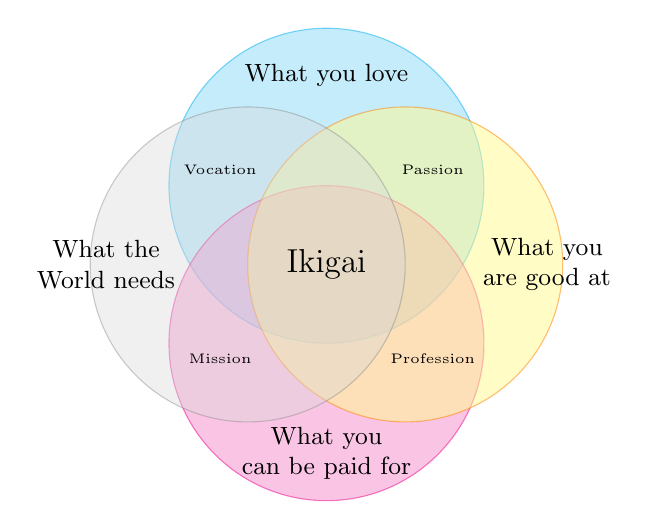
\begin{tikzpicture}
% Circles
\fill[cyan!45, opacity=0.5, draw=cyan] (0,1) circle (2cm);
\fill[magenta!45, opacity=0.5, draw=magenta] (0,-1) circle (2cm);
\fill[yellow!45, opacity=0.5, draw=orange] (1,0) circle (2cm);
\fill[black!15, opacity=0.4, draw=gray] (-1,0) circle (2cm);
% Labels
\node[font=\small, align=center] at (-2.8,0) {What the\\ World needs};
\node[font=\small, align=center] at (2.8,0) {What you\\ are good at};
\node[font=\small, align=center] at (0,-2.4) {What you\\ can be paid for};
\node[font=\small] at (0,2.4) {What you love};
% Small Labels
\node[font=\tiny] at (1.35,-1.2) {Profession};
\node[font=\tiny] at (1.35,1.2) {Passion};
\node[font=\tiny] at (-1.35,-1.2) {Mission};
\node[font=\tiny] at (-1.35,1.2) {Vocation};
% Title
\node[font=\large] at (0,0) {Ikigai};
\end{tikzpicture}
\end{document}
